\documentclass[10pt,twocolumn,letterpaper]{article}

\usepackage{cvpr}
\usepackage{times}
\usepackage{epsfig}
\usepackage{graphicx}
\usepackage{amsmath}
\usepackage{amssymb}

% Include other packages here, before hyperref.

% If you comment hyperref and then uncomment it, you should delete
% egpaper.aux before re-running latex.  (Or just hit 'q' on the first latex
% run, let it finish, and you should be clear).
\usepackage[breaklinks=true,bookmarks=false]{hyperref}

\cvprfinalcopy % *** Uncomment this line for the final submission

\def\cvprPaperID{****} % *** Enter the CVPR Paper ID here
\def\httilde{\mbox{\tt\raisebox{-.5ex}{\symbol{126}}}}

% Pages are numbered in submission mode, and unnumbered in camera-ready
%\ifcvprfinal\pagestyle{empty}\fi
\setcounter{page}{1}
\begin{document}

%%%%%%%%% TITLE
\title{Contextual String Embeddings for Sequence Labeling}
\author{Alan Akbik\\
zalando Research\\
Mühlenstraße 25\\
10243 Berlin\\
{\tt\small Alan Akbik@zalando.de}
\and
Duncan Blythe\\
zalando Research\\
Mühlenstraße 25\\
10243 Berlin\\
{\tt\small Duncan Blythe@zalando.de}
\and
Roland Vollgraf\\
zalando Research\\
Mühlenstraße 25\\
10243 Berlin\\
{\tt\small Riland Vollgraf@zalando.de}
% For a paper whose authors are all at the same institution,
% omit the following lines up until the closing ``}''.
% Additional authors and addresses can be added with ``\and'',
% just like the second author.
% To save space, use either the email address or home page, not both
}


\maketitle
%\thispagestyle{empty}

%%%%%%%%% BODY TEXT
\section{Introduction}
As a basic task and foundation work of NLP, sequence labeling has a significant
influence on the follow-up works, such as named entity recognition (NER), 
part-of-speech (PoS) tagging, etc. For the traditional machine learning methods, 
we initially use HMM (Hidden Markov Model) to solve the problem. Regarded the tag 
sequence as hidden state sequence and sentence as an obvious sequence, HMM calculates
the probability distribution of each moment by defining the 5-tuple flow (hidden state
set $S$, the observed value set $O$, state transition matrix $A$, initial state probability
distribution $\pi$, observed value probability distribution of specified state $B$).
Generally speaking, HMM involves two basic tasks, assessment and decoding. The assessment aims
to calculate the probability of the observed sequence, and it always adopts a backward or forward
algorithm. While decoding is required to ensure the most likely hidden state sequence
based on the obvious sequence, which is selects Viterbi algorithm. However, because
HMM determines each hidden states individually, rather than considering the dependency 
of interlink states, the result that labeling two or more prepositions simultaneously will 
happen in the part-of-speech tagging. To overcome this shortcoming, the simple way is to
add the connection matrix at adjacent hidden states, therefore, by improving maximum the 
entropy model, the CRF (Conditional random field) comes into being. Relying on hand-feature
descriptions, CRF applied widely at pre-deep learning era. With deep neural network rapidly
developed, depending on the powerful feature representation ability, BiLSTM+CRF 
took replace to CRF and renewed the record of sequence labeling.

About embeddings, the original form is one-hot discrete word vectors. Although this method 
is simplified, it exists a semantic gap and the curse of dimensionality. After that, the word bag 
model (counting the times of words in the files), TF-IDF (reflecting the proportion of the words in 
files). Based on the distributional hypothesis (the words have the similar means with the 
same context), Bengio et al. (2001) invented NNLM (Neural Network Language Model) and 
presented the word vector, which converts the one-hot code to the dense vectors by looking-up
operation and the look-up table is created by the training process. According to the input 
distinguish, word vector networks include NNLM, C$\&$W, CBOW, Skip-gram, etc. Comparing to the
NNLM, C$\&$W as well as Skip-gram delete the hidden layer and ignore the order of the words, making the
architecture slender. Besides, for the reason that the softmax calculation needs considerable 
computing resource and time, the researcher proposed hierarchical softmax, constructing the Huffman
tree to update the vocabulary partially. Furthermore, about the polysemy like "bank", we can
embedding multi-word vectors for different contexts, then using k-means clustering choose 
appropriate word vectors. Some experiments show concatenating different word vectors training
by different network architectures, such as RNN, CNN, LSTM, can also improve the F1 value.   

The biggest innovation of this paper about the sequence labeling task is to improve the tradition
embedding, the author propose to leverage the internal states of a trained character language 
model to produce a novel type of word embedding which referring to as contextual string embeddings.
These embeddings have the distinct properties that they (a) are trained without any explicit notion 
of words and thus fundamentally model words as sequences of characters, and (b) are contextualized 
by their surrounding text, meaning that the same word will have different embeddings depending on 
its contextual use.

%------------------------------------------------------------------------
\section{Major contributions and the proposed solutions}

Figure1. is the detailed structure of CLM,  use characters as atomic units of language modeling, 
allowing text to be treated as a sequence of characters passed to an LSTM which at each point in 
the sequence is trained to predict the next character1. This means that the model possesses a 
hidden state for each character in the sequence.

\begin{figure*}
	\begin{center}
		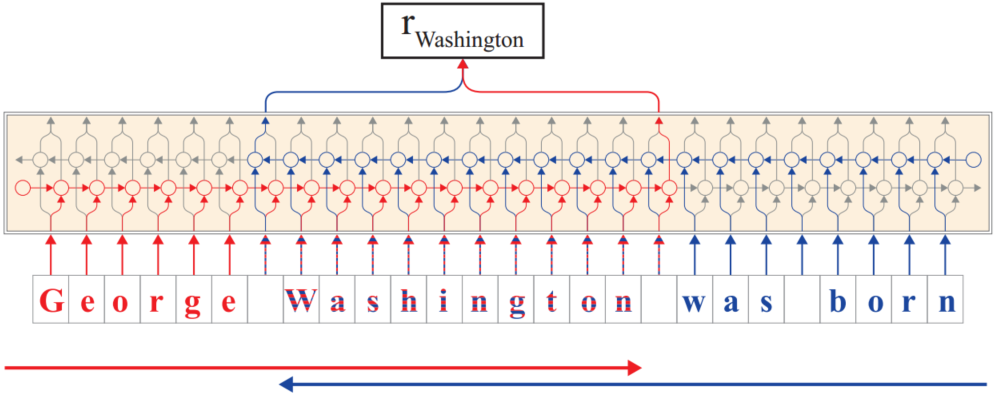
\includegraphics[width=.5\linewidth]{CRL.png}
	\end{center}
	\caption{Extraction of a contextual string embedding for a word (“Washington”) in a sentential 
	context. From the forward language model (shown in red), we extract the output hidden state after 
	the last character in the word. This hidden state thus contains information propagated from the
	beginning of the sentence up to this point. From the backward language model (shown in blue), 
	we extract the output hidden state before the first character in the word. It thus contains 
	information propagated from the end of the sentence to this point. Both output hidden states 
	are concatenated to form the final embedding.}
	\label{fig:short}
\end{figure*}

\begin{figure*}
	\begin{center}
		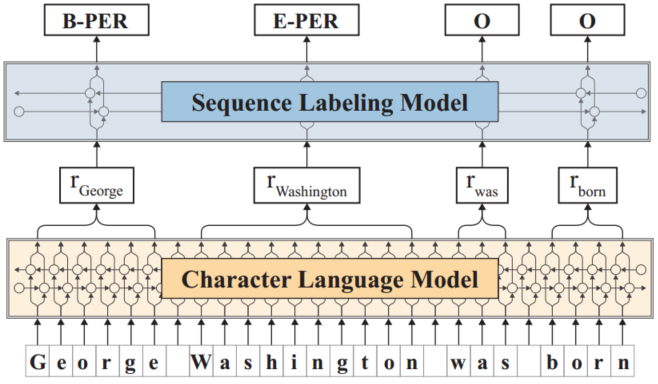
\includegraphics[width=.5\linewidth]{modelstructure.png}
	\end{center}
	\caption{High level overview of proposed approach. A sentence is input as a character sequence
		into a pre-trained bidirectional character language model. From this LM, we retrieve for 
		each word a contextual embedding that we pass into a vanilla BiLSTM-CRF sequence labeler, 
		achieving robust state-of-the-art results on downstream tasks (NER in Figure).}
	\label{fig:short}
\end{figure*}

Figure2. is the sequence labeling model detail. The network can split two parts, Character Language
Model (CLM) and Sequence Labeling Model (SLM). CLM leverages BiLSTM hidden state encoding word vectors,
on account of BiLSTM merges the context information naturally, thus it can  produce different embeddings 
for polysemous words depending on their usage and model words and context fundamentally as sequences 
of characters, to both better handle rare and misspelled words as well as model subword structures 
such as prefixes and endings. The CLM can be utilized to downstream sequence labeling tasks effectively. 
As for name entity recognition (NER), the author utilizes BiLSTM-CRF model.

Whatsmore, the author evaluate the proposed contextual string embedding in the five configurations: 
Proposed, Proposed+word, Proposed+char, Proposed+word+char, Proposed+all. The experiment shows that 
the added use of classic word embeddings in setup Proposed+word often produces the best results. 
Especially for NER, the use of classic word embeddings increases average F1 score by 1.1 pp to 93.07, 
compared with 91.97 for Proposed.

%------------------------------------------------------------------------
\section{Own understanding of the contributions and the unsolved problems of the paper}

Comprehensively, for the sequence labeling tasks, there are two mainstream methods currently, the 
first one is based on the abundant high-quality corpus to pre-training word vectors, like Bert, and 
the second one is based on the feature representation and selection ability of networks to extract the 
hidden state and embedding or concatenating various word vectors so as to improve results. 

\section{Detailed Information}
@inproceedings{akbik2018contextual,
	
	title={Contextual string embeddings for sequence labeling},
	
	author={Akbik, Alan and Blythe, Duncan and Vollgraf, Roland},
	
	booktitle={Proceedings of the 27th International Conference on Computational Linguistics},
	
	pages={1638--1649},
	
	year={2018}
}
\end{document}
